\documentclass[11pt, letterpaper, onecolumn]{article}

\usepackage[english]{babel}
\usepackage{soul}
\usepackage{mathtools}
\usepackage[utf8]{inputenc}
\usepackage{graphicx}
\usepackage{float}
\usepackage[german=quotes]{csquotes}
\usepackage{hyperref}
\usepackage{fancyhdr}
\usepackage{gensymb}
\usepackage{units}
\usepackage{hhline}
\usepackage{color}
\usepackage{titling}
\usepackage[normalem]{ulem}
\usepackage[margin=2.5cm]{geometry}
\usepackage{amsmath}
\usepackage{amssymb}
\usepackage{amsfonts}
\usepackage{pgfplots}
\usepackage{array}
\usepackage{makecell}
\usepackage{subfigure}
\usepackage{lipsum}
\usepackage{url}
\usepackage{relsize}

\begin{document}



\newgeometry{a4paper, left=20mm, right=20mm, top=30mm, bottom=30mm}
\definecolor{pantone294}{cmyk}{1,0.6,0,0.2}
\setlength{\columnsep}{6mm} 

\title{Revision Subproject 1.1: Time Evolution\\
        and\\
        \vspace{2mm}
        Subproject 1.2: Eigenvalues and Eigenvectors} 
\author{Florian Telleis / Florian Hollants / Mickey Wilke}
\date{\today}

\pagestyle{fancy}
\lfoot{Humboldt-Universität zu Berlin}
\rfoot{Revision Subproject 1.1} 
        \newgeometry{left=14mm, right=13.5mm, top=13.5mm, bottom=30mm}
	\begin{titlepage}
		\thispagestyle{empty}
		\begin{figure}
			
		\end{figure}
		\vspace*{-43mm}\hspace{-6mm}\textbf{\textcolor{pantone294}{\large{Mathematisch-Naturwissenschaftliche Fakultät}}}\\\\\\\\\\
		\textcolor{pantone294}{Institut für Physik}\\
		\vspace{30mm}
		\begin{center}
			\textcolor{pantone294}{\huge{Computational Physics II}}\\\vspace*{7mm}
			\textcolor{pantone294}{\huge{\textbf{\thetitle}}}\\\vspace*{10mm}
			\textcolor{pantone294}{\theauthor}\\\vspace*{10mm}
			\textcolor{pantone294}{\thedate}\\\vspace*{20mm}
			\begin{tabular}{ll}
				\textbf{Work Group:} & Albert Einstein	 \\ \\
				\textbf{Students:} & Florian Telleis (612716) \\
									& Florian Hollants (648689)\\
									& Mickey  Wilke (642815)\\ \\
				\textbf{Submitted:} & 07.01.2025 \\ \\				
			\end{tabular}
		\end{center}
	\end{titlepage}
	\makeatother
	\restoregeometry
		
		\newpage
	
	
	
	
	
	
	\tableofcontents
	
	
	
	
	
	\vspace{0.5cm}
	
	
	\section{How the code works}
	Before addressing the main changes, we quickly explain how to run the new code structure. To test the hamiltonian and integrators you can just run the files "test$\_$hamiltonian.py" and "test$\_$integrators.py", respectively. We wrote separate functions that run the defined tests and output tables. These functions are called by running the two files (one can change the information inside of the functions, change the input or only run one of the functions).\\
	To get the final animation you have to run the file "animation.py". To show you, the changes to our project files did not affect our animation in a meaningful way, we included the animation that was run with the revised code. \\ 
	Running the file "test$\_$integr$\_$converg.py" outputs the testing for the convergence of the integrators.
	
	
	\subsection{Modularity}
	Now, what changed explicitly regarding our first submission. As a first step, we improved our file management by implementing a modularity of files, dividing our prior one python file into seven (and of course more files for the second sub-project). The content of these modules did not change if not stated otherwise in the sections Variables, Tests or Convergence. \\
	The new file system is listed below: \\ 
	- "variables.py": defining variables and few general functions\\
	- "hamiltonian.py": defining potential and hamiltonian\\
	- "test$\_$hamiltonian.py": defining the tests for the hamiltonian and also running them for multiple $N$ and dimensions \\
	- "integrators.py": defining both the integrators \\
	- "test$\_$integrators.py": defining the tests for the integrators and also running them for multiple $N$ and dimensions \\
	- "test$\_$integr$\_$converg.py": testing the dependence of the integrators on $M$ or rather $\tau$ \\
	- "animation.py": defining functions for animation and animating


\subsection{Variables}
	We then changed/deleted all our old variables depending on other parameters to be now only defined by dimensionless values, without changing their value in regards to our first submission. In our case of modularity, where we work with the same variables in multiple python files, it is practical to store these global variables (and some basic functions used in multiple other files) in an extra python file. We can then import these global variables by "from variables import *". \\
	This change worked with most of the prior functions and tests. Except, when needing to change certain variables of a function in a separate file from where the function is defined, which means the change of variable is not possible in a separate file. Explicitly, what changed: \\
	\textbf{1.} For the new hamiltonian tests (see section 1.4), we had to change our definition of the potential to take $N$ from the size of the given array instead of using the global $N$.\\
	\textbf{2.} A second change regarding the hamiltonian file was done. We defined potential$\_$variable and \\hamilton$\_$variable which are the same as our old potential and hamiltonian but take $\mu$ and $\epsilon$ as an input for the convergence of eigenvalues/-vectors in the second sub-project, where we have to change these.\\
	\textbf{3.} Similarly, but for the first sub-project, for testing the integrators in dependence of $M$ or rather $\tau$, we had to add an additional input for $\tau$ into the integrators (and therefore the tests). Thus, the dependence could be evaluated without having to define the integrators in the same file as the tests, which was falsely done in our first submission.


	\subsection{Tests}
	The tests we included in the sub-project 1.1 were in general not modified for this revision. But we added proper executions for these tests: we now run these tests of the hamiltonian and integrators for multiple dimensions and $N$. Here we focus on $N$ = 5, 10, 15 and 20; because the relevance of boundary conditions and resulting errors decrease for large $N$. The exact output for running the testing files is shown in the following figures for each of the $N$ for 4 dimensions (hamiltonian) and 3 dimensions (integrators, due to long run-time). The tests include "randomly" generated arrays. Therefore these tests run 10 times each and depending on the criteria the maximum error of each test is saved.\\
	Also notice that the output in the following figures shows $N$ as a float, it is an integer nonetheless.
	\\
	\\
        \newpage
        \noindent
	In figure \ref{fig:test-hamiltonian} the tests of linearity, hermiticity and positivity of the hamiltonian and test      for the eigenvectors of the kinetic hamiltonian are shown.
	\begin{figure} [H] 
	\begin{center}
	\includegraphics[width=15cm]{"test_hamiltonian2.png"}
	\caption{Output of our test functions for the hamiltonian for multiple $N$ and $D$; 10 iterations.} 	\label{fig:test-hamiltonian}
	\end{center}	
	\end{figure}
	\\
    \noindent
	One can see that the errors for testing the linearity are in the range of $10^{-14}$, where for higher dimensions the error increases. It also seems that for higher $N$ the errors increase. But in some cases this could also be due to the "random" generation of input arrays. But, we observe this same dependence for the hermiticity with errors up to $10^{-10}$ and eigenvectors with errors up to $10^{-12}$. The positivity of the hamiltonian was correct for all iterations.
    \newpage
        \\
	\\
	Now the integrator tests, which can be seen in figure \ref{fig:test-integrators}. 
	\begin{figure} [H] 
	\begin{center}
	\includegraphics[width=13cm]{"test_integrators2.png"}
	\caption{Output of our test functions for the integrators for multiple $N$ and $D$; 10 iterations.} \label{fig:test-integrators}
	\end{center}
	\end{figure}
	\\
	The errors of unitarity for the strang-splitting integrator and linearity for both of the integrators are in the range of $10^{-16}-10^{-15}$, which is even smaller than for the hamiltonian tests and checks with the expectation. The unitarity errors for the second-order integrator are far larger even in 1D with $10^{-5}$ and rising for higher dimensions. Even greater errors can be seen for the energy conservation tests. This is expected as energy conservation is not given for these integrators. The important detail however, is that no significant lowering of errors for higher $N$ is seen, which is most likely due to $N=20$ still being relatively small and using randomly generated arrays, which change the error maxima.
	\\
	\\
	Below, all the tests were run for one iteration for $N=5$ and $D=9$ as an additional testing. In figure \ref{fig:test-hamiltonian-9D} for the hamiltonian tests and in figure \ref{fig:test-integrators-9D} for the integrator tests.\\
    One can see the same behaviour as above, just exaggerated. \\
	With all these evaluated results, we can safely conclude that our tests (correctly) run in more dimensions than $D=1$, even for small $N$.
	\begin{figure} [H] 
	\begin{center}
	\includegraphics[width=6cm]{"test_hamiltonian-9D2.png"}
	\caption{Output of our test functions for the hamiltonian for $N=5$ and $D=9$; 1 iteration.} \label{fig:test-hamiltonian-9D}
	\end{center}
	\end{figure}
	\begin{figure} [H] 
	\begin{center}
	\includegraphics[width=7cm]{"test_integrators-9D2.png"}
	\caption{Output of our test functions for the integrators for $N=5$ and $D=9$; 1 iteration.} \label{fig:test-integrators-9D}
	\end{center}
	\end{figure}
	
	
	
	
	
	
	
	\subsection{Convergence of the Integrators}
	We are interested in seeing how certain quantities behave for different values of $M$ and therefore different values of $\tau$. We will look at $\Delta E$ for both integrators, as well as the deviation of the norm for the second-order integrator, and lastly, we will look at the average difference between the two integrators. For that we will take a specific time $T$ and calculate the time evolution of one specific state in $M$ steps up to that time $T$. Afterwards, we repeat the same process for different values of $M$.\\
    Since both integrators use approximations that improve with smaller values of $\tau$, we expect the deviation of the norm and energy to decrease with increasing $M$. Lets look at the second order integrator first: $U(t,0)=1-i\hat{H}\hat{\tau}-\frac12\hat{H}^2\hat{\tau}^2$
    \begin{align*}
        \braket{\psi_t|\psi_t}&=\bra{\psi_0}[U^\dagger(t,0)U(t,0)]^M\ket{\psi_0}\\
        &=\bra{\psi_0}\left[1+\frac{1}{4}\hat{H}^4\hat{\tau}^4 \right]^M\ket{\psi_0}\\
        &=\bra{\psi_0}1+\frac{M}{4}\hat{H}^4\hat{\tau}^4+\mathcal{O}(\hat{\tau}^6)\ket{\psi_0}\\
        &\approx \braket{\psi_0|\psi_0}+\frac{\hat{T}\hat{E}_0^4}{4}\hat{\tau}^3\braket{\psi_0|\psi_0}\\
        \implies \Delta|\psi_t|^2&\sim\hat{\tau}^3\sim M^{-3}
    \end{align*}
    Now we look at the strang-splitting integrator: $U(t,0)=e^{-i\frac{\hat{V}\hat{\tau}}{2}}e^{-i\hat{K}\hat{\tau}}e^{-i\frac{\hat{V}\hat{\tau}}{2}}$
    \begin{align*}
        U(t,0)&=e^{-i\frac{\hat{V}\hat{\hat{\tau}}}{2}}e^{-i\hat{K}\hat{\hat{\tau}}}e^{-i\frac{\hat{V}\hat{\hat{\tau}}}{2}}\\
        &=(1-i\hat{\tau}\frac{V}{2}-\frac{1}{2}\left(\hat{\tau}\frac{V}{2}\right)^2+\frac{i}{6}\left(\hat{\tau}\frac{V}{2}\right)^3)(1-i\hat{\tau} K-\frac{1}{2}\left(\hat{\tau} K\right)^2+\frac{i}{6}\left(\hat{\tau} K\right)^3)(1-i\hat{\tau}\frac{V}{2}-\frac{1}{2}\left(\hat{\tau}\frac{V}{2}\right)^2+\frac{i}{6}\left(\hat{\tau}\frac{V}{2}\right)^3)\\&+\mathcal(O)(\hat{\tau}^4)\\
        &=1-i\hat{\tau} H-\frac{1}{2}\hat{\tau}^2(K^2+V^2+KV+VK)\\&+\frac{i\hat{\tau}^3}{6}\left(8\left(\frac{V}{2} \right)^3 + 3K\left(\frac{V}{2} +\right)^2 + 3\left(\frac{V}{2} \right)^2K +3K^2\frac{V}{2}+3\frac{V}{2}K^2 +6\frac{V}{2}K\frac{V}{2}+K^3 \right) +\mathcal{O}(\hat{\tau}^4)\\
        &=e^{-iH\hat{\tau}}+\mathcal{O}(\hat{\tau}^3)
    \end{align*}
Therefore we can conclude that
\begin{align*}
    \braket{\psi_t|\psi_t}&=\bra{\psi_0}U^\dagger U\ket{\psi_0}\\
    &=\bra{\psi_0}((e^{iH\hat{\tau}}+\mathcal{O}(\hat{\tau}^3))(e^{-iH\hat{\tau}}+\mathcal{O}(\hat{\tau}^3)))^M\ket{\psi_0}\\
    &=\bra{\psi_0}(1+\mathcal{O}(\hat{\tau}^3))^M\ket{\psi_0}\\
    &=\braket{\psi_0|\psi_0}+\bra{\psi_0}M\mathcal{O}(\hat{\tau}^3)\ket{\psi_0}\\
    &=\braket{\psi_0|\psi_0}+\bra{\psi_0}\mathcal{O}(\hat{\tau}^2)\ket{\psi_0}
\end{align*}
We therefore expect $\Delta|\psi_t|^2\sim\hat{\hat{\tau}}^2\sim M^{-2}$
	\begin{figure} [H] 
	\begin{center}
	\includegraphics[width=16cm]{"final_loglog_1.png"}
	\caption{log-log plots against M with slopes [-3.0198987799444197, -1.9999479182661908, -3.009455253603387, -2.004740059443111]}
	\end{center}
	\end{figure}
    \noindent
	The calculated slopes align with our predicted scaling.
 	(noch die neue Animation reinpacken um zu zeigen dass modular funktioniert?)




	\newpage

    \rfoot{Subproject 1.2} 

   
	\section{How the code works for the second sub-project}	
	The following segment of the report deals with the second-subproject. The code is built from the following modules:\\
    1. "eigenmethods.py", the conjugate-gradient and power method functions are defined here\\
    2. "test\_eigenmethods.py", the tests of the aforementioned functions are defined and can be run in this module\\
    3. "convergence\_eigenmethods.py", this module contains the functions for the infinite volume and continuum limit test\\
	
	
	
	\section{Workflow}
	This section will explain our workflow for the different parts of our code.
    \\
    \\
        \underline{\textbf{Conjugate-gradient and Arnoldi method}}
    \\
    \\
    We started by implementing the simple power method as discussed in the lecture. This is not documented in the code, since we only need the Arnoldi method. Building on the power method we implemented the Arnoldi algorithm. This required the implementation of the Gram-Schmidt algorithm. We noted that errors occurred quite frequently during testing when we chose the starting vectors carelessly. The vectors need to be linearly independent. This issue was permanently fixed though when the Krylov space was added, which ensures linear independence(as long as we don't start with an eigenvector). At this stage we already decided to build the Arnoldi, and later the conjugate-gradient method, using the Hamiltonian from our first subproject. \\
    \\
    In hindsight this was not the best choice. Introducing the matrix as another variable into the Arnoldi function would have been useful for debugging purposes. We have chosen the stopping criterion in the Arnoldi function such that the error on every eigenvalue  falls below the given error. We also defined a function for performing all matrix-vector operations called "matrix\_multi" outside of the Arnoldi function. This is useful because it will be the only piece of code which needs to connect the Arnoldi function to the conjugate gradient method.\\
    \\
    xxxximplementing conjugate gradientxxxxx
    \\
    \\
        \underline{\textbf{Testing the Algorithm}}
    \\
    \\
    We decided on the following tests for the eigenvalue/eigenvector algorithm:\\
    1. Testing our implementation of the conjugate-gradient method by checking if it actually calculates the inverse of the Hamiltonian. This error should fall below our chosen tolerance. \\
    2. Checking the orthonormality of the calculated eigenvectors functions as a test for the implemented Gram-Schmidt algorithm. Verifying this is especially necessary because we also need to gauge the error created by Gram-Schmidt.\\
    3. By simply calculating both sides of the eigenvalue equation we can effectively test our algorithm. We expect the error to be larger than our tolerance, because of the added deviations from the conjugate-gradient method. To see these errors is very important in order to choose a fitting tolerance for the required accuracy.\\
    \\
    4. Lastly we used the idea of the Rayleigh-Ritz method to verify that our calculated eigenvalue is truly the smallest. This can be done by changing the corresponding eigenvector by an arbitrarily small amount and calculating the eigenvalue. The Eigenvalue should not become any smaller than the one we calculated.\\
    We considered other tests such as using standard-library linear algebra programs for comparison. We decided against that, since this would require turning our Hamiltonian into a matrix which is exactly what we do not want to do in this project. 
    \\
    \\
        \underline{\textbf{Infinite volume and continuum limit}}
    \\
    \\   
    Next we needed to investigate the accuracy of our algorithm for the infinite volume case. This is done by studying if and when the eigenvalues start to converge regarding $N$. After deciding on a value of $N>240$ we approached the continuum limit by finding a suitable way to implement it, see \ref{continuum}. xxxxsomething regarding the parityxxxxx
	
	
	\section{Implementing conjugate-gradient and power method}
	


	
	
	\section{Testing}
	The tests in this section are done in a similar fashion as in the first sub-project. Meaning, that we code separate tests for our functions, which are the conjugate gradient and Arnoldi method. These can then be used with varying parameters (e.g. $N$ and tolerance) to evaluate different behaviours. Notice, this is not the task of convergence of eigenvalues/eigenvectors but the needed preparation for this part to ensure correct results. \\
	Two important aspects to add: 1. We ran all tests multiple times with different parameters, the tests shown in this chapter are therefore a distinct selection to underline noticed effects. 2. The figures in this chapter do not have a detailed description, as the important information is given in the caption of the figure/in the figure itself and it would just be too much text cluttering.

	\subsection{Conjugate-gradient}
	We start with testing our implementation of the conjugate gradient method. Our method does not calculate explicitly the inverse of the hamiltonian but the inverse multiplied with a vector $v$ or in code language $H^{-1}(v)$. In this way, we never have to write $H$ as a matrix (same as in sub-project 1.1) but can use the hamilton function acting on $v$. Therefore, we can simply test if our result is actually inverse by calculating $v-H(H^{-1}(v))\thickapprox 0$ and output the maximum error of all the array elements. The conjugate gradient method is also implemented to work in multiple dimensions. A test for multiple $N$ and $D$ is shown in figure \ref{fig:test_inverse-ND}. A following test for multiple tolerances and max iterations is shown in figure \ref{fig:test_inverse-tol}.
	\begin{figure} [H] 
	\begin{center}	
	\includegraphics[width=17cm]{"test_inverse_ND2 better.png"}
	\caption{Test for the conjugate gradient method for multiple $N$ and $D$; 20 iterations with each time a "randomly" generated array $v$ being tested. Output: maximum error and as a second element the number of times the maximum iterations (maxiters) were reached.} \label{fig:test_inverse-ND}
	\end{center}
	\end{figure}
	\begin{figure} [H] 
	\begin{center}	
	\includegraphics[width=19cm]{"test_inverse_tolMax.png"}
	\caption{Test for the conjugate gradient method for multiple tolerances and max iterations; 100 iterations with each time a "randomly" generated array $v$ being tested. Output: maximum error and as a second element the number of times the maximum iterations (maxiters) were reached. Notice: when every iteration reaches the maxiters (does not converge) we set the error to 0 as a place-holder!} \label{fig:test_inverse-tol}
	\end{center}
	\end{figure}
	\\
	With these test results, we can conclude that our conjugate gradient method correctly converges to the inverse for high enough max iterations, with an error depending on the prior set tolerance. The implementation even works in multiple dimensions.
	
	
	\subsection{Orthonormality and Ritz}
	Furthermore, we can test our implementation of the Arnoldi method, which uses the conjugate gradient and power method. Both have a tolerance and max iteration, which are kept the same for both methods.\\
	First, we check if the first four calculated eigenvectors are really orthonormal. This is done for different $N$ and tolerances of the Arnoldi method. The starting vector $v$ is generated via "np.ones($N$)" and the test is shown in figure \ref{fig:test_orth}.\\
	One observes that the orthonormality test outputs exceptionally low errors in the range of $10^{-16}-10^{-15}$.
	\begin{figure} [H] 
	\begin{center}	
	\includegraphics[width=19cm]{"test_eigen_orth-tol.png"}
	\caption{Test for orthonormality of first 4 eigenvectors calculated via the Arnoldi method, for multiple $N$ and tolerances. Output: maximum error of all the different array elements.} \label{fig:test_orth}
	\end{center}
	\end{figure}
	\\
	\\
	As a second test, we implemented the Rayleigh-Ritz method to check if the calculated lowest eigenvalue is in fact the lowest possible eigenvalue. The test is done for the lowest (first) eigenvalue and the second lowest (second) eigenvalue and corresponding eigenvector. We vary the tolerance of Arnoldi and the starting deviations of the Ritz method. The output is the number of times the studied eigenvalue was not the smallest. The iterations of the tests are done by increasingly lowering the starting deviation. We also did multiple tests for different $N$ but chose to show the results for a starting vector $v$ of "np.ones(220)". Though, the important aspect that the first eigenvalue is always the smallest was always true. The results can be seen in figure \ref{fig:test_ritz}.
	\begin{figure} [H] 
	\begin{center}	
	\includegraphics[width=19cm]{"test_ritz-N220-dev0.01.png"}
	\caption{Testing the two lowest eigenvalues with Ritz method for eigenvalues/vectors calculated via the Arnoldi method for multiple starting deviations of Ritz and tolerances of Arnoldi. The red rectangles show the only parameter changing between the three tests. Output: number of times the studied eigenvalue was not the smallest one.} \label{fig:test_ritz}
	\end{center}
	\end{figure}
	\\
	The Ritz method always outputs the first eigenvalue as the lowest, as expected. This cannot be said for the second lowest eigenvalue, again, as expected. Why the count at the last test for the second eigenvalue at $tolerance=10^{-7}$ is not 100 but 11 is not clear, but this could be a random artefact at these exact parameters.
	
	
	\subsection{Eigenvalue equation}
	As a last step, we evaluate the eigenvalue equation that can be calculated with the eigenvalues/vectors from the Arnoldi method and the hamiltonian. This is done by looking at the maximum error of all the array elements between the two sides of the eigenvalue equation.\\
	We start with an initial vector of "np.ones($N$)" with multiple $N$ and different tolerances for the Arnoldi method. This first test is shown in figure \ref{fig:test_eigen_ones}.
	\begin{figure} [H] 
	\begin{center}	
	\includegraphics[width=19cm]{"test_eigen.png"}
	\caption{Testing the eigenvalue equation for the four lowest eigenvalues/vectors calculated via the Arnoldi method for multiple $N$ ($v$=np.ones($N$)) and tolerances. Output: maximum error of the eigenvalue equation for each of the four eigenvalues} \label{fig:test_eigen_ones}
	\end{center}
	\end{figure}
	\\
	With an initial guess of $v$=np.ones($N$), one can see that to achieve an error of $<1\%$ for the eigenvalues we would need to have tolerances of $10^{-9}$. As for $10^{-7}$ and $N=200$ the error of the fourth eigenvalue/vector is $1,66\%$. But after careful analysis of the hamiltonian and starting conditions, we found that the four lowest eigenvalues are not the bland four lowest calculated eigenvalues for a random initial guess but the output of our Arnoldi method is dependent on the initial guess. You can read more deeply into this discussion in the next section of convergence! Without interfering with the argumentation of the next section, we can already test the new initial guesses. This will be an even and odd starting vector, where each the lowest and second lowest eigenvalue is degenerate for these two initial guesses. Which together make up our four lowest eigenvalues.\\
	Thus, we have to test the same parameters as in figure \ref{fig:test_eigen_ones} with both of the new initial guesses but only for the two lowest eigenvalues each. The first tests were done by using randomly generated functions, which were odd or even. But this randomness meant that depending on the starting vector, we could get a good convergence below our set tolerance, or we would run into the max iterations. These were the results from extensive tests.  We now use odd and even vectors build with ones. The results can be seen in figure \ref{fig:test_eigen_even-odd}.
	\begin{figure} [H] 
	\begin{center}	
	\includegraphics[width=19cm]{"test_eigen_even-odd.png"}
	\caption{Testing the eigenvalue equation for an odd and even starting vector of ones; for each the two lowest eigenvalues/vectors are calculated via the Arnoldi method for multiple $N$ and tolerances. Output: maximum error of the eigenvalue equation} \label{fig:test_eigen_even-odd}
	\end{center}
	\end{figure}
	\\
	We now observe for a tolerance of $10^{-7}$ errors of smaller than $1\%$ for all eigenvalues and $N$, which was our wanted limit.
	\\
	\\
	As a final but small test, we just look if our input of the numbers of eigenvalues the Arnoldi method has to calculate has any influence on the calculation itself. A simple comparison can bee seen in figure \ref{fig:test_eigen_number}. As one can observe, the change results in no difference.
	\begin{figure} [H] 
	\begin{center}	
	\includegraphics[width=19cm]{"test_eigen_numbers.png"}
	\caption{The lowest eigenvalues from calculation via the Arnoldi method and errors of the eigenvalue equation for the 4 lowest and 10 lowest eigenvalues.} \label{fig:test_eigen_number}
	\end{center}
	\end{figure}
		\\
		\\
		With all these tests from the different sections, we can conclude that our functions do work as expected under the condition of choosing the right conditions. This means we take an even and odd starting vector for which we only calculate the two lowest eigenvalues. Because of this, we can set the tolerances to $10^{-7}$ and for every $N$ still have errors of smaller than $1\%$. The important aspect is to also set the maximum iterations high enough to not run into an error.\\
		With this meaningful work done, we can advance to furthermore analyse the behaviour of eigenvalues and eigenfunction under convergence in the next section.
	

 	\section{Convergence of eigenvalues/eigenvectors}
	Before taking the infinite volume limit and the continuum limit we will make use of symmetry properties of our hamiltonian to improve on our method of calculating the lowest eigenvalues and their corresponding eigenvectors.

	\subsection{Parity}
 	The Parity operator takes any function $\psi(x)$ from the hilbert space and returns $\mathbb{P}\psi(x)=\psi(-x)$. The operator has the two degenerate eigenvalues $\pm1$ which correspond to symmetric (even) and antisymmetric (odd) functions. Using the symmetry of our potential $V(x)=V(-x)$ we can show, that the parity operator commutes with the hamiltonian.
  	\begin{align*}
		[\hat{H},\hat{\mathbb{P}}]f(x)&=\hat{H}f(-x)-\hat{\mathbb{P}}\left(-\frac{\hbar^2}{2ma^2}\sum\limits_k\left(f(x+ae_k)+f(x-ae_k)-2f(x)\right)+V(x)f(x) \right)\\
	    &=-\frac{\hbar^2}{2ma^2}\sum\limits_k\left(f(-x+ae_k)+f(-x-ae_k)-2f(-x)\right)+V(x)f(-x)\\&+\frac{\hbar^2}{2ma^2}\sum\limits_k\left(f(-x+ae_k)+f(-x-ae_k)-2f(-x)\right)-V(-x)f(-x)\\
	    &=0
	\end{align*}
 	From this result follows, that we can simultaneously diagonalize both operators, meaning that any eigenvector of one operator has to be an eigenvector of the other operator as well. Being an eigenvector of the parity operator means, that $\psi(x)=\pm\psi(-x)$, the eigenvectors have to be either even or odd!\\
	Now we want to use this result to improve the arnoldi method. To do this, we make the observation that applying the hamiltonian operator to an even/odd function will return an even/odd function again. This can be shown by doing the explicit calculation, or by reasoning about the fact that an even/odd function is automatically an eigenvector of the parity operator. We want to show that $f(x)=\pm f(-x)\implies (\hat{H}f)(x)=\pm(\hat{H}f)(-x)$:
 	\begin{align*}
    		(\hat{H}f)(-x)&=\hat{\mathbb{P}}(\hat{H}f)(x)=\hat{H}(\hat{\mathbb{P}}f)(x)=\pm(\hat{H}f)(x)
	\end{align*}
 	Since the arnoldi-method consists of repeatedly applying the hamiltonian operator we can see, that using an even/odd vector as a starting guess ensures that we only find even/odd solutions, reducing the space of possible eigenvectors drastically, and since we know all eigenvectors of the hamiltonian must be even/odd we can be sure, that we aren't missing any.\\
  	The advantage of using this idea is a drastically improved runtime of the code since the arnoldi-method converges faster.


  
 	\subsection{Infinite Volume Limit}
  	We first try to do the infinite volume limit, by using the arnoldi-method twice; once for an even starting guess and one for an odd guess. For reproducability purposes we didn't choose a random starting vector, but instead used only one, minus one and zero in the middle. We initially chose a fixed value of $\mu=20$, $\varepsilon=\frac{1}{60}$ and $N=41$. Then we repeat that process for bigger values of $N$ and plotted the eigenvalues against $N$. We chose only odd numbers for $N$, since it is easier to generate the even and odd starting guesses that way.
    	\begin{figure} [H] 
	\begin{center}
	\includegraphics[width=15cm]{"inf_vol_lim_final.png"}
	\caption{Eigenvalues of the of the Hamiltonian for different values of $N$}
	\end{center}
	\end{figure}
	The eigenvectors seem to have converged from $N=201$ onwards although two of the four eigenvalues seem to have vanished. Zooming in on one the lower dot reveals, that the two eigenvalues are much closer compared to the distance to the other two eigenvalues. Since we don't expect the eigenvalues to change much anymore, we say that the infinite volume limit is well approximated for $N>240$. 
 	\begin{figure} [H] 
	\begin{center}
	\includegraphics[width=15cm]{"eigenvectors_Parity.png"}
	\caption{Eigenvectors for $N=241$ with $\mu=20$ and $\varepsilon=\frac{1}{60}$, plotted against $n\varepsilon=\frac{x}{r}$ using parity}
	\end{center}
	\end{figure}
 	First we notice, that the eigenvectors are exclusively real. This is, because we have chosen a real starting vector for the arnoldi method, which in return only produces real eigenvectors, since the hamiltonian has no imaginary part. We could have started with a complex starting vector, and gotten complex eigenvectors as well, but since we can multiply any eigenvector by a complex phase without changing the fact that it is still an eigenvector of the operator, we would have been able to generate the purely real eigenvectors from there as well.\\
  	We can also visualize how the Eigenvectors changed with increasing values of $N$.

   	\begin{figure} [H] 
	\begin{center}
	\includegraphics[width=15cm]{"inf_vol_lim_N41.png"}
	\caption{Eigenvectors for $N=41$ with $\mu=20$ and $\varepsilon=\frac{1}{60}$ plotted against $n\varepsilon=\frac{x}{r}$ using parity}
	\end{center}
	\end{figure}
 	
 	\begin{figure} [H] 
	\begin{center}
	\includegraphics[width=15cm]{"inf_vol_lim_N81.png"}
	\caption{Eigenvectors for $N=81$ with $\mu=20$ and $\varepsilon=\frac{1}{60}$ plotted against $n\varepsilon=\frac{x}{r}$ using parity}
	\end{center}
	\end{figure}

 	\begin{figure} [H] 
	\begin{center}
	\includegraphics[width=15cm]{"inf_vol_lim_N121.png"}
	\caption{Eigenvectors for $N=121$ with $\mu=20$ and $\varepsilon=\frac{1}{60}$ plotted against $n\varepsilon=\frac{x}{r}$ using parity}
	\end{center}
	\end{figure}

 	\begin{figure} [H] 
	\begin{center}
	\includegraphics[width=15cm]{"inf_vol_lim_N161.png"}
	\caption{Eigenvectors for $N=161$ with $\mu=20$ and $\varepsilon=\frac{1}{60}$ plotted against $n\varepsilon=\frac{x}{r}$ using parity}
	\end{center}
	\end{figure}

 	\begin{figure} [H] 
	\begin{center}
	\includegraphics[width=15cm]{"inf_vol_lim_N201.png"}
	\caption{Eigenvectors for $N=201$ with $\mu=20$ and $\varepsilon=\frac{1}{60}$ plotted against $n\varepsilon=\frac{x}{r}$ using parity}
	\end{center}
	\end{figure}
	
	\subsection{Continuum Limit}
    	We want to look at the continuum limit in the infinite volume case. To do that we have to take the limit for $a\rightarrow0$. We have two variables that depend on $a$: $N=\frac{L}{a}$ and $\epsilon=\frac{a}{r}$. Since we only work with the dimensionless variables, we have to take the limit for $N\rightarrow\infty$ and $\epsilon\rightarrow0$ in such a way, that $N\epsilon=\frac{L}{r}=const$. To be in the infinite volume limit we will use $N\epsilon=\frac{241}{60}$. We will then make a list of multipliers $m\geq1$ and use values for $N=241*m$ and $\epsilon=\frac{1}{60\cdot m}$, we then plot the Eigenvalues against the different multipliers.
	\begin{figure} [H] 
	\begin{center}
	\includegraphics[width=15cm]{"cont_lim_final.png"}
	\caption{Eigenvalues of the hamiltonian for $N=mN_0$, $\varepsilon=\frac{\varepsilon_0}{m}$, $N_0=241$, $\varepsilon_0=\frac{1}{60}$ against $m$}
	\end{center}
	\end{figure}
	We can see, that the Eigenvalues have converged to the continuum limit from the very beginning, meaning the eigenvalues and vectors we found in the infinite volume limit, were already also converged in the continuum limit. While this result might be a little surprising, the starting value for $\varepsilon$ was chosen to be the same as we chose when making the animation of the wavefunction in the potential. In order to make that simulation work, we had to adjust the parameters accordingly. So when we settled on $N=200$ and $\varepsilon=\frac{1}{60}$ for the animation, since we found that those values worked well for it, we chose values for the infinite volume and continuum limit already.\\
	Therefore the Eigenvalues in the infinite volume, continuum limit ($N=241$, $\mu=20$, $\varepsilon=\frac{1}{60}$) are [0.48652252 1.39727169 0.48653768 1.39893003]. 


	
	
	



%	\hyperref[Quellen]{$^{[1]}$}	



	
%		\begin{figure} [h] 
%	\begin{center}
%	\subfigure[CGM]{\includegraphics[width=0.45\textwidth]{799px-Constant_current.svg.png}}
%    \subfigure[CHM]{\includegraphics[width=0.45\textwidth]{799px-Constant_height.svg.png}}
%\caption{Verschiedene Modi für das RTM Abrastern, entnommen aus \hyperref[Quellen]{[3]}}
%	\end{center}
%	\end{figure}


	

	
	%	\begin{figure} [h] 
%	\begin{center}
%	\includegraphics[width=8.8cm]{"QBER(R).jpg"}
%	\caption{QBER($R_{det}$) for three different photon sources and different attenuations; the data points are linearly connected for better visibility}
%	\end{center}
%	\end{figure}
	
	
	

%	\hyperref[Quellen]{$^{[1]}$}	

	
	
\newpage
	

	
%\section{Sources and Literature} \label{sources}
%
%		$[1]$ \textit{Titel} - Autor; (Vers.) Datum
%\vspace{0.4cm}
%		 \\
%		$[2]$ Internetseite: \textit{Titel} \\ \url{Link} \\- zuletzt besucht am Datum um Zeit
%		\vspace{0.4cm}
%		 \\
		
		
%		$[1]$ \textit{Titel} - Autor; (Vers.) Datum
%\vspace{0.4cm}
%		 \\
%		$[2]$ Internetseite: \textit{Titel} \\ \url{Link} \\- zuletzt besucht am Datum um Zeit
%		\vspace{0.4cm}
%		 \\

	
	

	
%\section{Appendix} \label{sec:appendix}

%	\begin{figure}[h]	
%	\begin{center}	
%	\subfigure[Random input wavefunction]{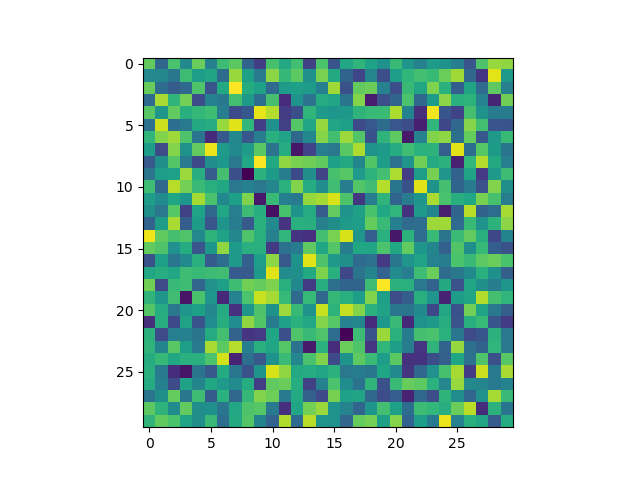
\includegraphics[width=0.35\textwidth]{function1_ABS.png}}
%    \subfigure[Potential]
%    {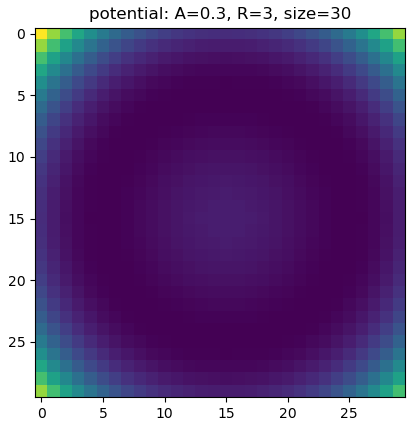
\includegraphics[width=0.35\textwidth]{potential2.png}}
%    \subfigure[Second-order integration]
%    {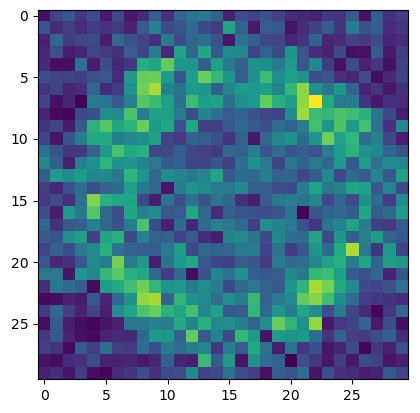
\includegraphics[width=0.35\textwidth]{so-integrator1_ABS.png}}
%	\caption{Tests with (a) random 2D wavefunction, (b) resulting potential and (c) the following time evolution with the second-order integrator after a certain amount of time steps M (not known anymore, but around 2000 with T=2)}
%	\label{fig:2D-so_integr}
%	\end{center} 
%	\end{figure}
	
	




	
\end{document}
